\chapter{Chapter 2}

\section{Model simulations of surprisal}
A direct measure of reaction time can be through `surprisal'; a quantity that measures how much any given node (in the modular graph of Figure \ref{fig:modular_graph}) that is visited is expected to be visited. Simply put, if a visited node is surprising, response times may be higher. This effect is observed in prior literature where surprisal is measured as $log k$ where $k$ is the number of connections in the node prior to the current node. \cite{lynn2020human} found that for this surprisal significantly impacted reaction times for a full length of random walk.

While all nodes in the graph used have the sam number of connections, a similar model of surprisal was used to simulate potential differences between the model. Briefly, since each cell $i, j$ in a row $i$ of the SR/TCM matrix represents the relative activation of the node associated with that column, a surprisal measure was computed as a $log M_{ij}$ of that cell.

\begin{figure}
    \centering
    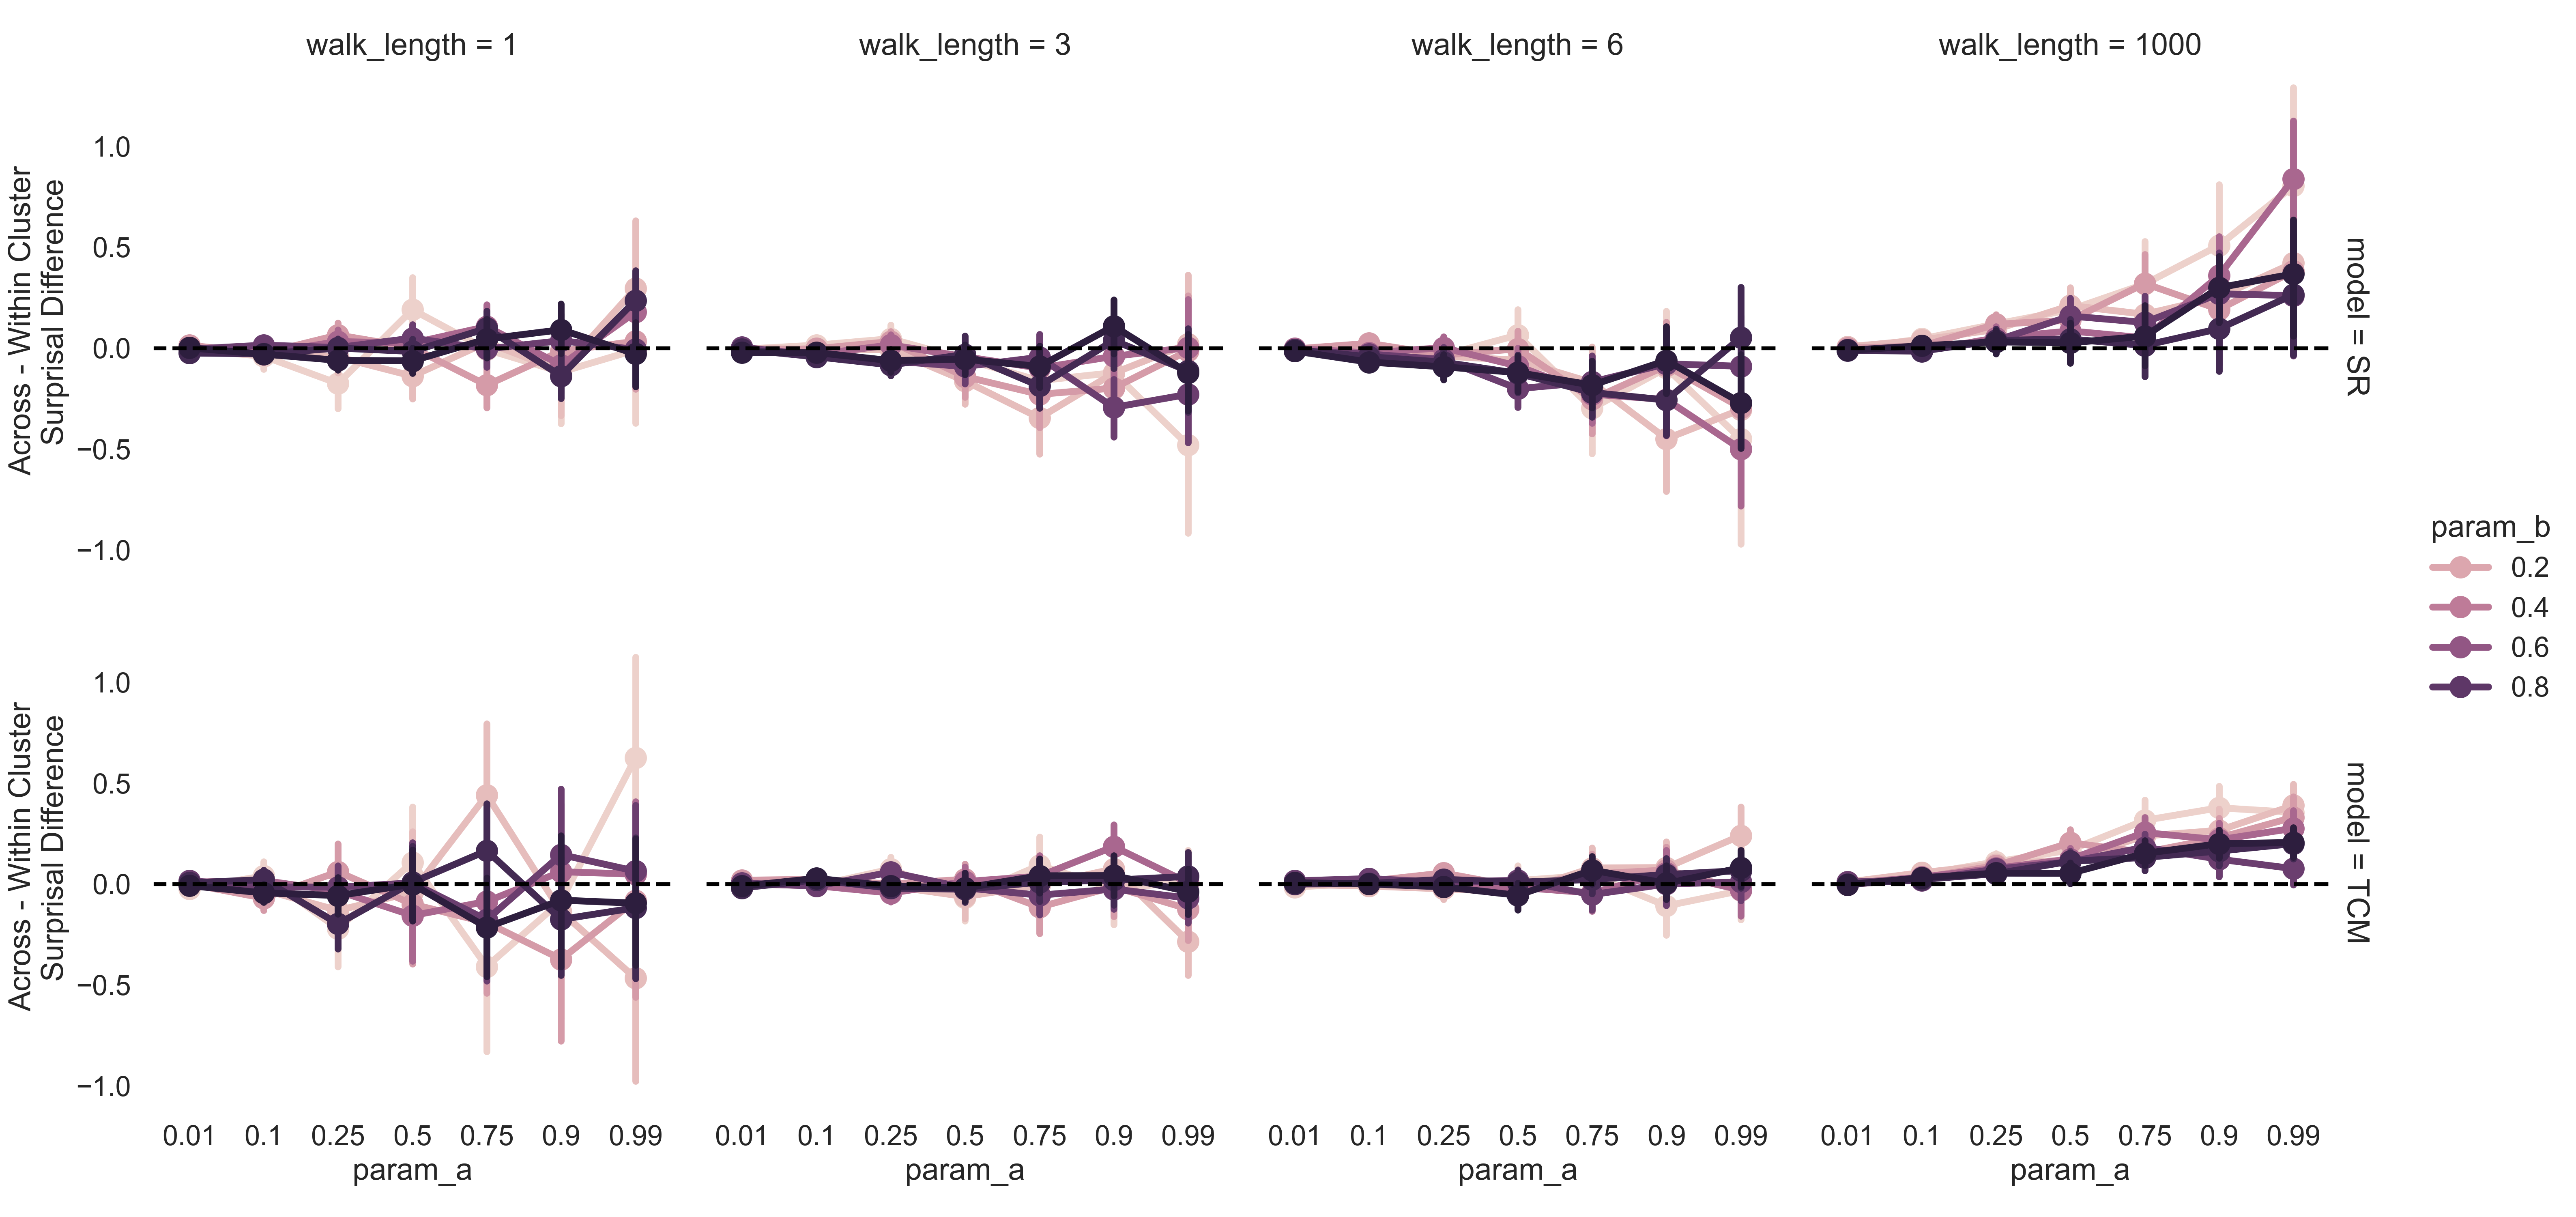
\includegraphics[width = \textwidth]{chapter_notebooks/chapter_2/figures/SR_TCM_walklength_boundary_nonboundary_surprisaldiff.png}
    \caption{Surprisal differences between cross-cluster and within-cluster transitions across walk lengths for representations generated by both SR (top row) and TCM (bottom row) models.}
    \label{fig:surprisal-sims}
\end{figure}

As Figure \ref{fig:surprisal-sims} shows, first surprisal across cluster increases with increased walk length. Second, there are no qualitative differences across possible parameter values in the effect of surprisal. For that reason, this measure of surprisal was not used to assess the models.


\section{Comparing first and the last blocks}

Similar to comparisons done in the main text, the response times between the boundary and non boundary nodes for the first and last blocks were compared when transitions leading into those nodes were within cluster (i.e. from another non-boundary nodes).

\begin{figure}[H]
    \centering
    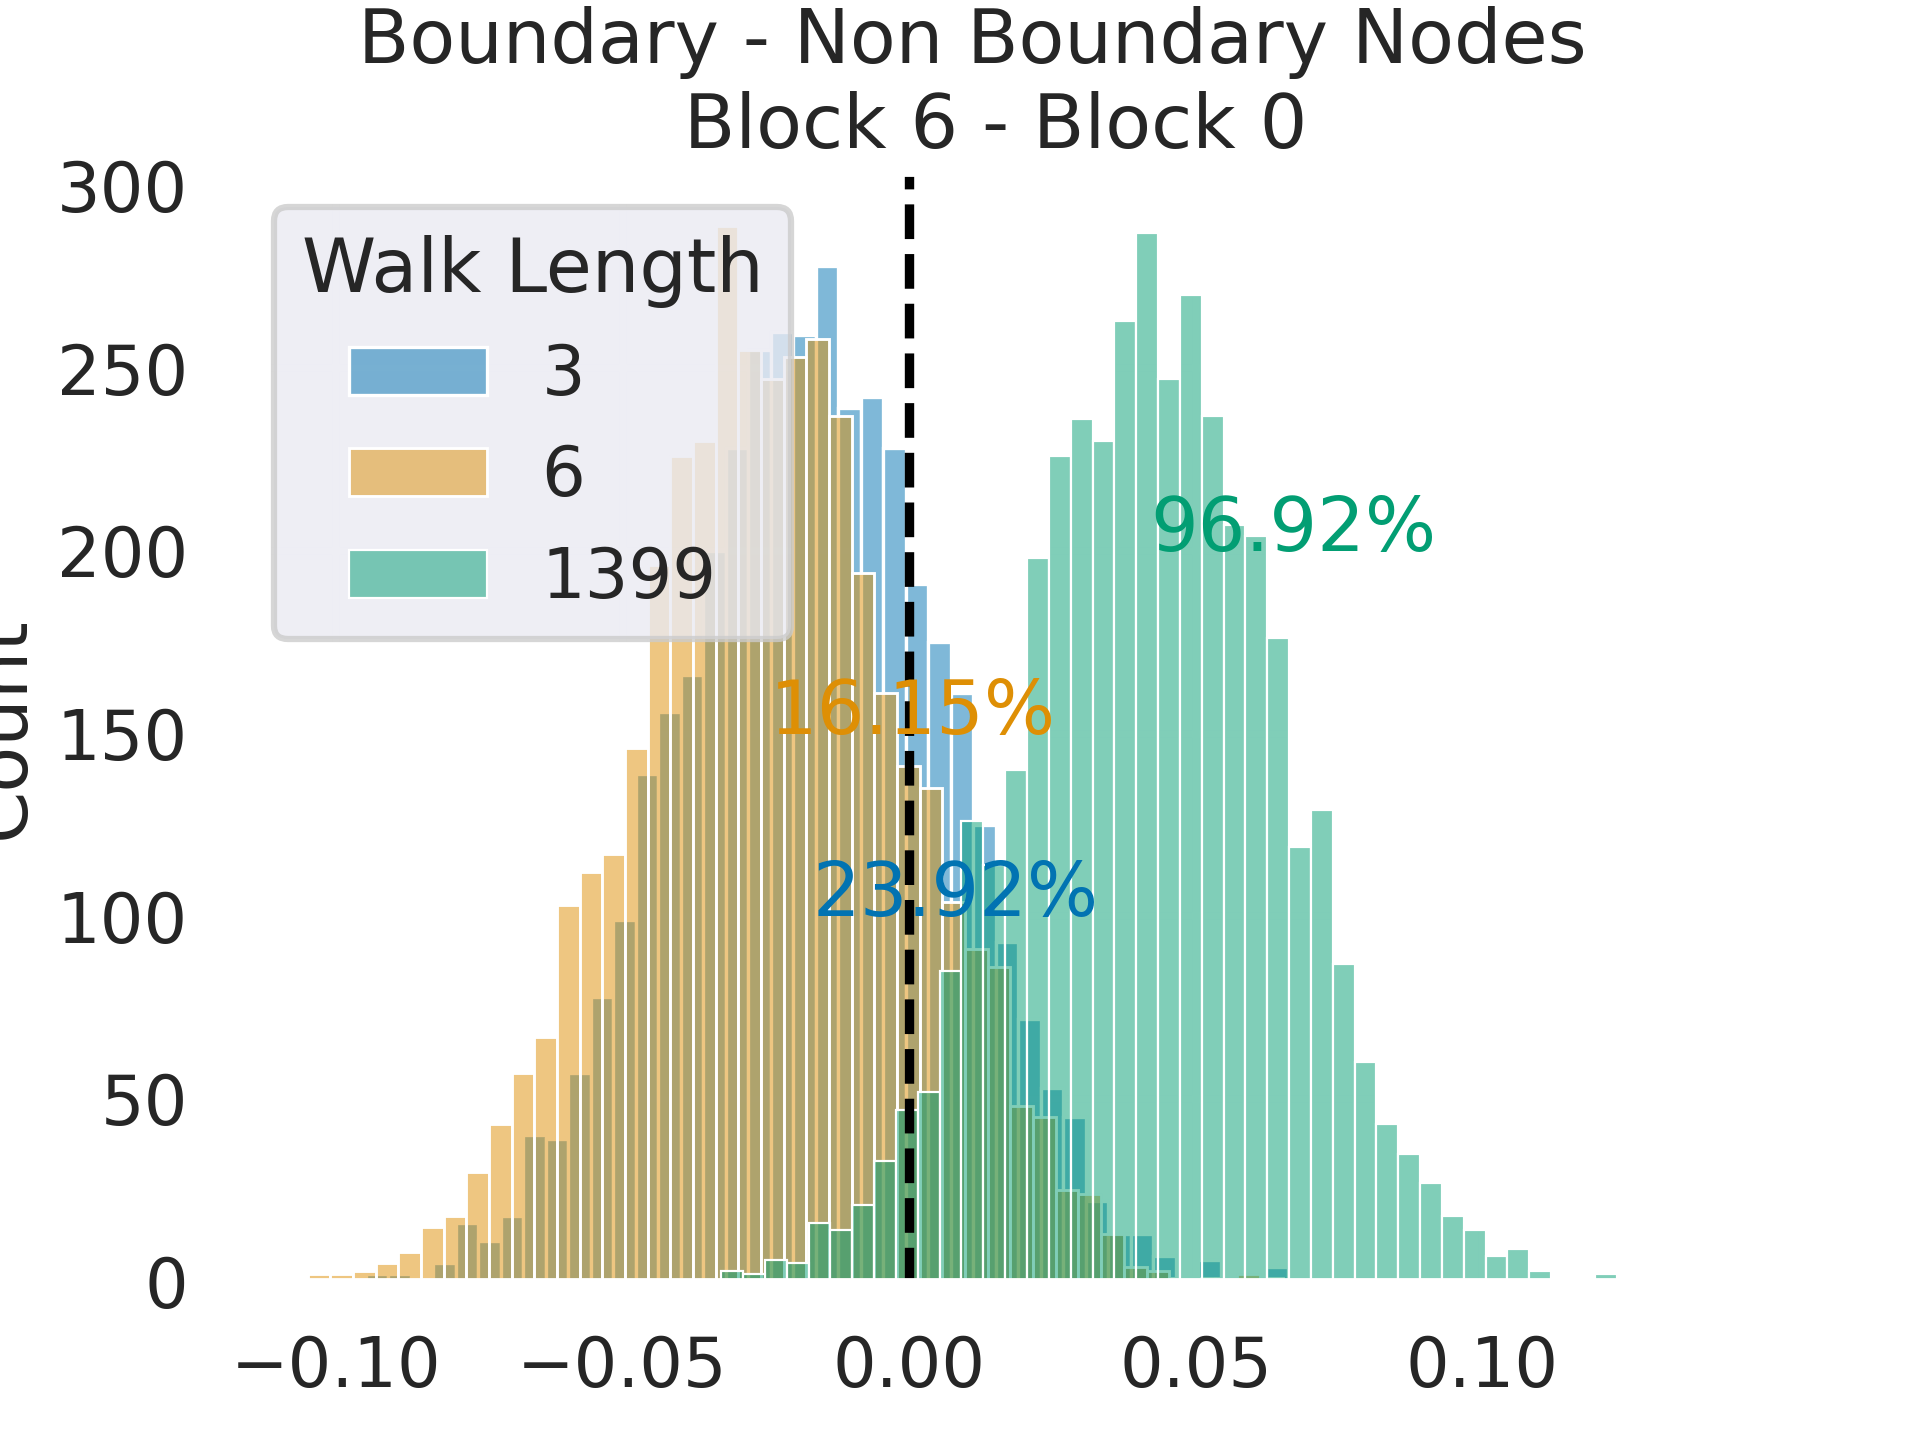
\includegraphics[width = 0.75\textwidth]{chapter_notebooks/chapter_2/figures/nb_b_diff_block60.png}
    \caption{Posterior estimates of comparisons the slowed down reaction times for boundary nodes relative to non boundary nodes. Reaction times slowed down more with larger walk lengths.}
    \label{fig:bayesmodel-firstlastblocks}
\end{figure}

Figure \ref{fig:bayesmodel-firstlastblocks} provides further evidence in support of the SR model. Reaction times decrease across the board. The decrease is lower for boundary nodes than non boundary nodes and this difference increases with walk length providing support for the SR model. 

\section{Fitting the entire learning curve}
The entire learning curve was fit using a linear model to estimate differences in decreased response times between boundary and non boundary nodes over time. 

\begin{figure}[H]
    \centering
    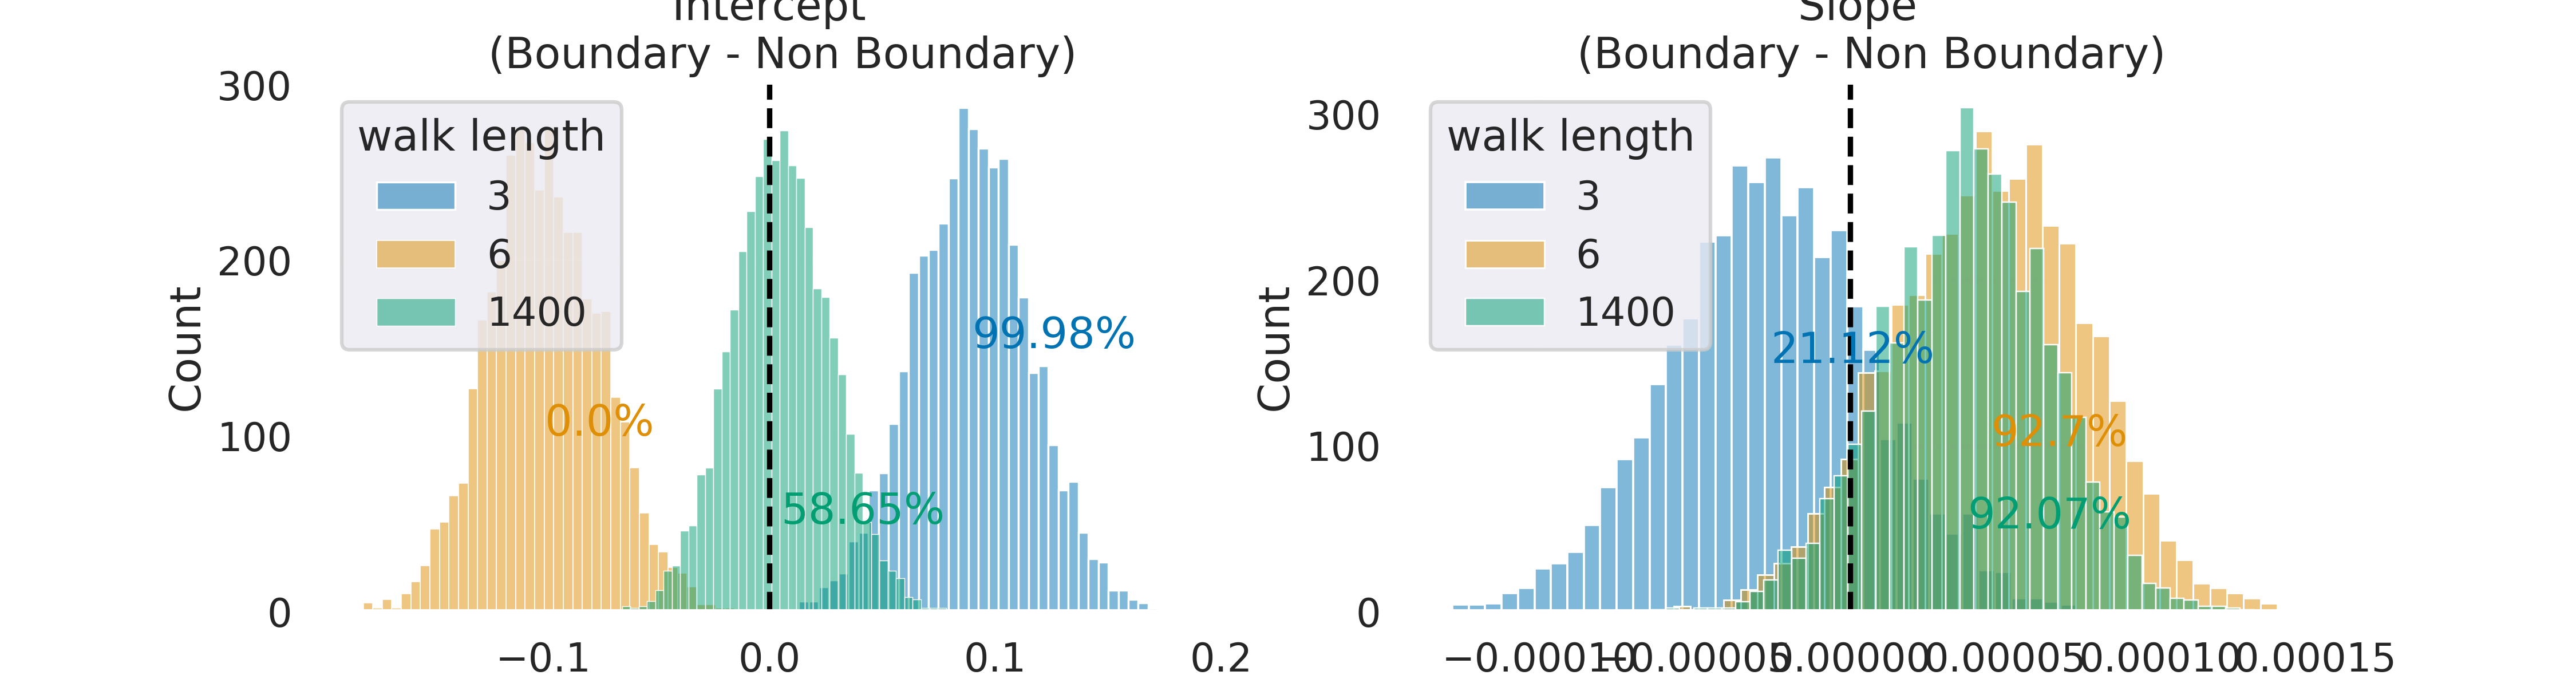
\includegraphics[width = \textwidth]{chapter_notebooks/chapter_2/figures/allblocks_lrmodel_trial_ppt_lag.png}
    \caption{Intercept (\textit{Left panel}) and Slope (\textit{Right panel}) differences of the linear model fit to all trials.}
    \label{fig:alltrial-lrmodel}
\end{figure}

As shown in figure \ref{fig:alltrial-lrmodel}, boundary and non boundary intercepts differed across walk lengths. This difference is likely due to randomly assigned response keys. The key metric of differences is the reduction in response times over time as measured by the slopes. As expected (from the SR model), walk lengths of 3 and 1399 lead to slower decrease in response times for boundary nodes than non boundary nodes (when transitioned to from another within cluster (non boundary) node). 

Interestingly, it appears that these slope differences are not meaningfully different between walk lengths of 6 and 1399. However, the findings reported in the main text (Figure \ref{fig:bayesmodel-firsttwoblocks}), it is likely that these differences were apparent earlier in the learning process for the walk length of 1399 than for walk length of 6. Conflicting results with the main text likely implies a need for a more complex model (such as a dual rate model \parencite{mcdougle2015explicit, smith2006interacting, savalia2022leap}) which allows for a quick initial decrease in reaction times followed by a slow asymptote. Future modeling work should investigate the impact of walk lengths on different aspects of the learning process. 
 

\begin{figure}[H]
    \centering
    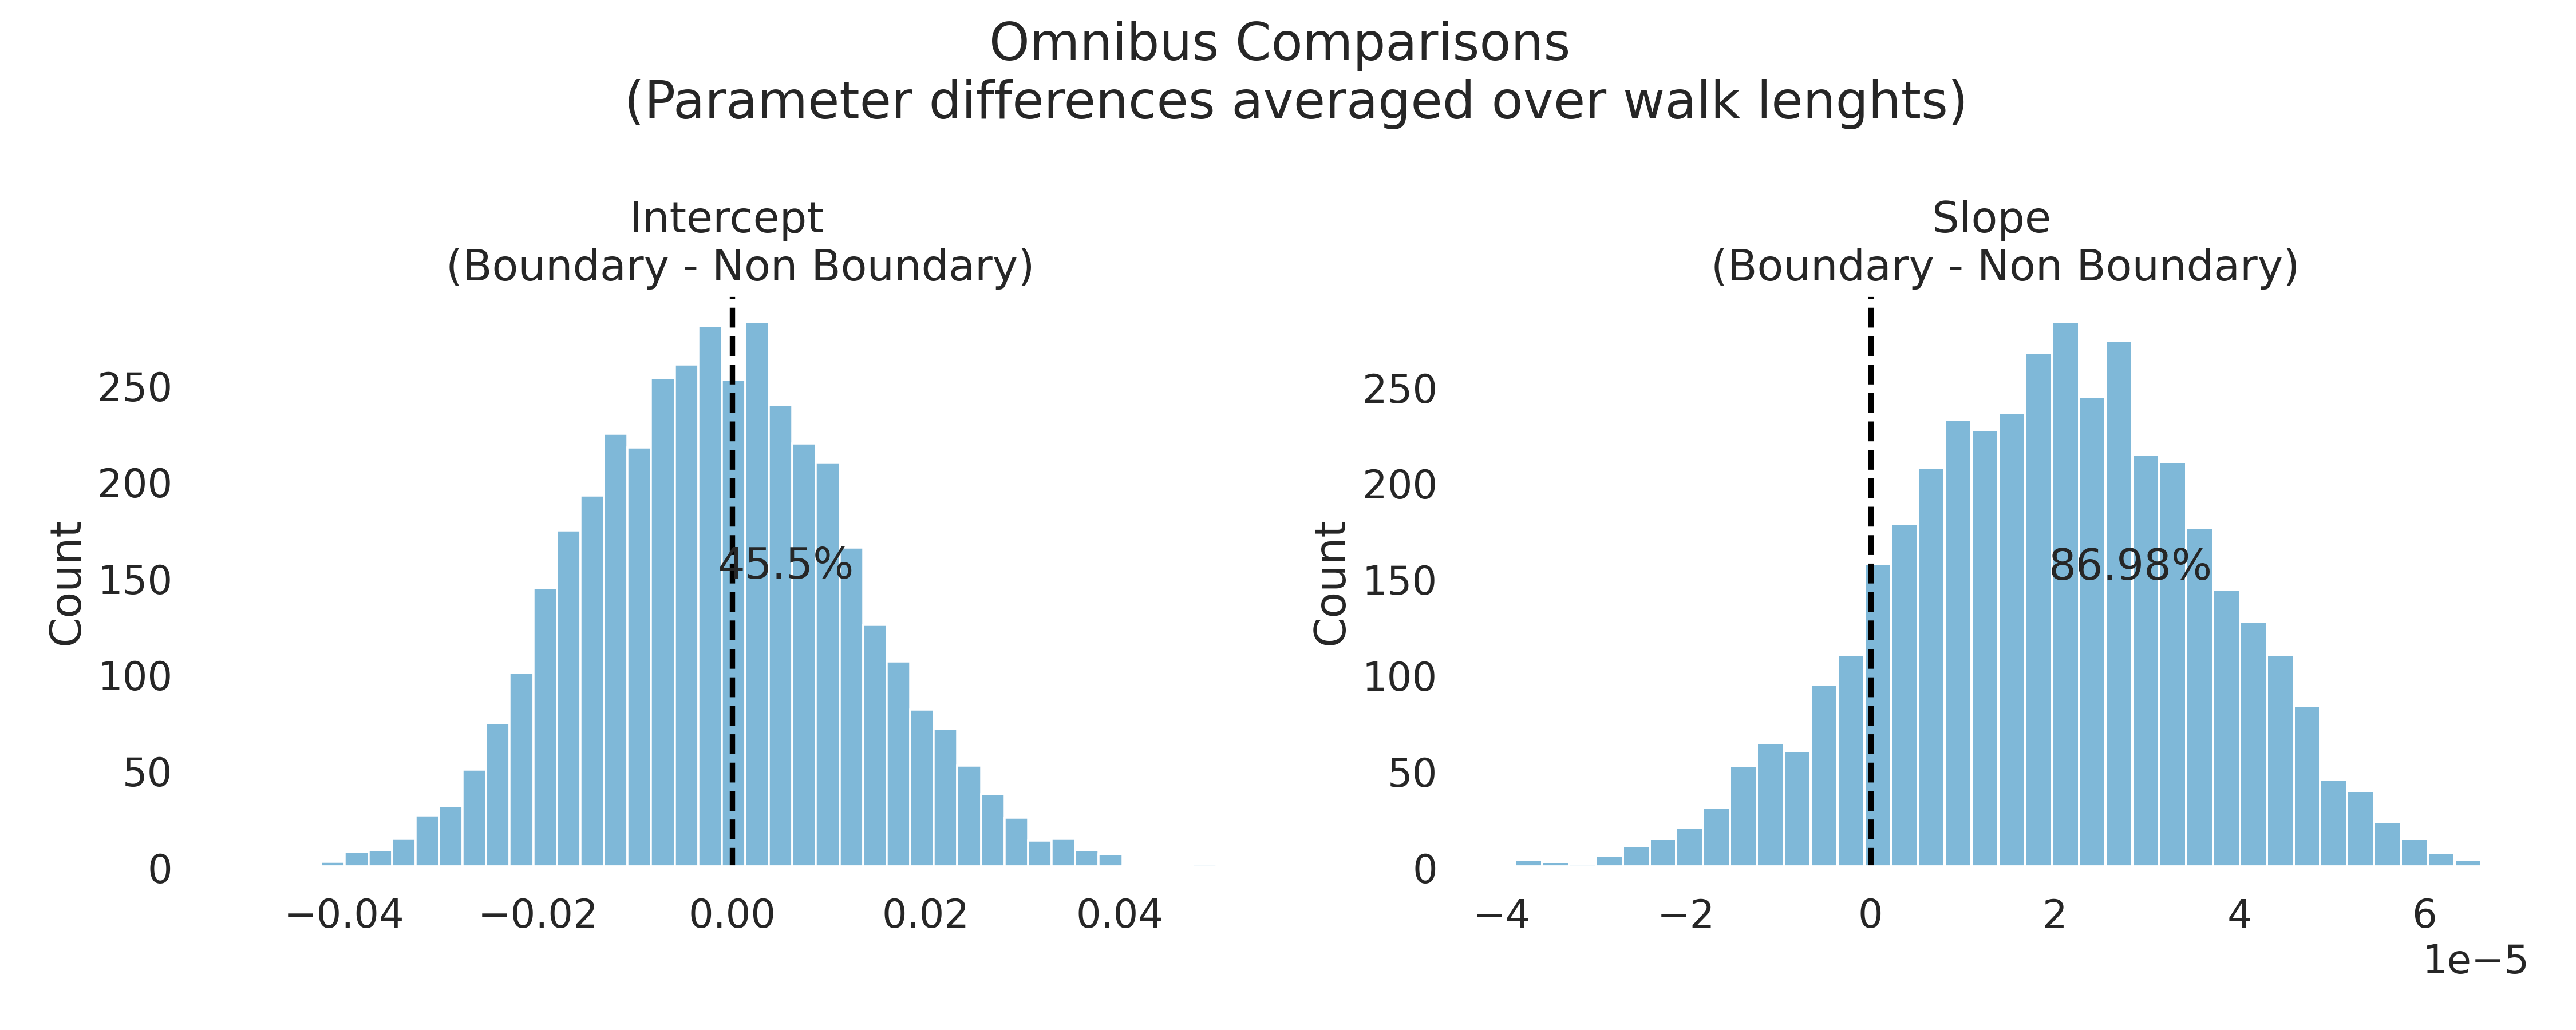
\includegraphics[width = \textwidth]{chapter_notebooks/chapter_2/figures/omnibus_comparisons_trialmodel.png}
    \caption{Omnibus comparisons between boundary and non-boundary nodes for linear models fit to all trials.}
    \label{fig:omnibus-alltrial-lrmodel}    
\end{figure}

Finally, Figure \ref{fig:omnibus-alltrial-lrmodel} presents comparisons between intercepts and slopes averaged across all walk lengths. Overall, boundary and non-boundary intercepts are largely similar (45\% samples above 0), however the average slope for boundary nodes is larger than that for the non-boundary nodes indicating response times to non-boundary nodes decrease faster than that to boundary nodes. 

\section{Model Statistics}

\subsection*{Stats for comparisons between the RTs for the first two blocks}

\begin{table}[H]
    \centering
    \begin{tabular}{lrrrr}
        \toprule
         & mean & sd & hdi 2.5\% & hdi 97.5\% \\
        \midrule
        beta block[0.0] & -0.066 & 0.176 & -0.409 & 0.269 \\
        beta block[1.0] & -0.080 & 0.177 & -0.417 & 0.271 \\
        beta lag & 0.039 & 0.007 & 0.026 & 0.053 \\
        beta transition exp & -0.018 & 0.004 & -0.025 & -0.011 \\
        beta trial ntr[boundary, 0.0] & -0.555 & 0.024 & -0.602 & -0.508 \\
        beta trial ntr[boundary, 1.0] & -0.629 & 0.028 & -0.685 & -0.574 \\
        beta trial ntr[non-boundary, 0.0] & -0.596 & 0.023 & -0.639 & -0.548 \\
        beta trial ntr[non-boundary, 1.0] & -0.650 & 0.028 & -0.702 & -0.596 \\
        \bottomrule
        \end{tabular}        
        \caption{Posterior parameter statistics for model fit to walk length 3 data comparing the first two blocks}
        \label{tab:first-two-blocks-3}
\end{table}

\begin{table}[H]
    \centering
    \begin{tabular}{lrrrr}
        \toprule
         & mean & sd & hdi 2.5\% & hdi 97.5\% \\
        \midrule
        beta block[0.0] & 0.143 & 0.173 & -0.191 & 0.482 \\
        beta block[1.0] & 0.124 & 0.181 & -0.225 & 0.475 \\
        beta lag & 0.043 & 0.008 & 0.028 & 0.058 \\
        beta transition exp & -0.031 & 0.004 & -0.038 & -0.023 \\
        beta trial ntr[boundary, 0.0] & 0.252 & 0.033 & 0.190 & 0.319 \\
        beta trial ntr[boundary, 1.0] & 0.184 & 0.037 & 0.111 & 0.257 \\
        beta trial ntr[non-boundary, 0.0] & 0.316 & 0.033 & 0.252 & 0.383 \\
        beta trial ntr[non-boundary, 1.0] & 0.241 & 0.037 & 0.165 & 0.310 \\
        \bottomrule
    \end{tabular}
    \caption{Posterior parameter statistics for model fit to walk length 6 data comparing the first two blocks}
    \label{tab:first-two-blocks-6}
\end{table}

\begin{table}[H]
    \centering
    \begin{tabular}{lrrrr}
        \toprule
         & mean & sd & hdi 2.5\% & hdi 97.5\% \\
        \midrule
        beta block[0.0] & -0.043 & 0.172 & -0.378 & 0.294 \\
        beta block[1.0] & -0.076 & 0.177 & -0.427 & 0.267 \\
        beta lag & 0.066 & 0.007 & 0.053 & 0.080 \\
        beta transition exp & -0.010 & 0.003 & -0.016 & -0.005 \\
        beta trial ntr[non-boundary, 0.0] & -0.476 & 0.023 & -0.522 & -0.431 \\
        beta trial ntr[non-boundary, 1.0] & -0.635 & 0.027 & -0.688 & -0.581 \\
        beta trial ntr[boundary, 0.0] & -0.499 & 0.024 & -0.546 & -0.455 \\
        beta trial ntr[boundary, 1.0] & -0.602 & 0.027 & -0.655 & -0.548 \\
        \bottomrule
        \end{tabular}   
        \caption{Posterior parameter statistics for model fit to walk length 1399 data comparing the first two blocks}
        \label{tab:first-two-blocks-1399}    
\end{table}

\subsection*{Stats for comparisons between the RTs for the first and last blocks}

\begin{table}[H]
    \centering
    \begin{tabular}{lrrrr}
        \toprule
         & mean & sd & hdi 2.5\% & hdi 97.5\% \\
        \midrule
        beta block[0.0] & -0.070 & 0.173 & -0.392 & 0.274 \\
        beta block[6.0] & -0.100 & 0.172 & -0.431 & 0.236 \\
        beta lag & 0.029 & 0.006 & 0.017 & 0.041 \\
        beta transition exp & -0.007 & 0.002 & -0.010 & -0.003 \\
        beta trial ntr[boundary, 0.0] & -0.561 & 0.020 & -0.601 & -0.523 \\
        beta trial ntr[boundary, 6.0] & -0.704 & 0.037 & -0.778 & -0.634 \\
        beta trial ntr[non-boundary, 0.0] & -0.604 & 0.020 & -0.642 & -0.563 \\
        beta trial ntr[non-boundary, 6.0] & -0.730 & 0.039 & -0.808 & -0.656 \\
        \bottomrule
    \end{tabular}        
    \caption{Posterior parameter statistics for model fit to walk length 3 data comparing the first and the last blocks}
    \label{tab:first-last-blocks-3}    
\end{table}

\begin{table}[H]
    \centering
    \begin{tabular}{lrrrr}
        \toprule
         & mean & sd & hdi 2.5\% & hdi 97.5\% \\
        \midrule
        beta block[0.0] & -0.054 & 0.175 & -0.406 & 0.279 \\
        beta block[6.0] & -0.099 & 0.178 & -0.460 & 0.228 \\
        beta lag & 0.038 & 0.006 & 0.026 & 0.050 \\
        beta transition exp & -0.006 & 0.002 & -0.010 & -0.003 \\
        beta trial ntr[boundary, 0.0] & -0.538 & 0.019 & -0.574 & -0.501 \\
        beta trial ntr[boundary, 6.0] & -0.734 & 0.038 & -0.809 & -0.660 \\
        beta trial ntr[non-boundary, 0.0] & -0.528 & 0.020 & -0.568 & -0.489 \\
        beta trial ntr[non-boundary, 6.0] & -0.700 & 0.038 & -0.777 & -0.629 \\
        \bottomrule
    \end{tabular}
    \caption{Posterior parameter statistics for model fit to walk length 6 data comparing the first and the last blocks}
    \label{tab:first-last-blocks-6}    
    
\end{table}

\begin{table}[H]
    \centering
    \begin{tabular}{lrrrr}
        \toprule
         & mean & sd & hdi 2.5\% & hdi 97.5\% \\
        \midrule
        beta block[0.0] & -0.053 & 0.178 & -0.404 & 0.306 \\
        beta block[6.0] & -0.122 & 0.176 & -0.458 & 0.230 \\
        beta lag & 0.060 & 0.006 & 0.049 & 0.072 \\
        beta transition exp & -0.003 & 0.001 & -0.006 & -0.001 \\
        beta trial ntr[non-boundary, 0.0] & -0.515 & 0.019 & -0.553 & -0.478 \\
        beta trial ntr[non-boundary, 6.0] & -0.845 & 0.034 & -0.910 & -0.778 \\
        beta trial ntr[boundary, 0.0] & -0.538 & 0.020 & -0.576 & -0.499 \\
        beta trial ntr[boundary, 6.0] & -0.825 & 0.034 & -0.891 & -0.762 \\
        \bottomrule
    \end{tabular}        
    \caption{Posterior parameter statistics for model fit to walk length 1399 data comparing the first and the last blocks}
    \label{tab:first-last-blocks-1399}    
\end{table}


\subsection*{Parameter statistics for linear model including all trials}

\begin{table}[H]
    \centering
    \begin{tabular}{lrrrr}
        \toprule
         & mean & sd & hdi 2.5\% & hdi 97.5\% \\
        \midrule
        alpha ntr[3, boundary] & 0.466 & 0.138 & 0.215 & 0.760 \\
        alpha ntr[3, non-boundary] & 0.376 & 0.138 & 0.106 & 0.650 \\
        alpha ntr[6, boundary] & 0.440 & 0.138 & 0.166 & 0.699 \\
        alpha ntr[6, non-boundary] & 0.539 & 0.138 & 0.261 & 0.789 \\
        alpha ntr[1400, boundary] & 0.489 & 0.134 & 0.281 & 0.826 \\
        alpha ntr[1400, non-boundary] & 0.484 & 0.133 & 0.263 & 0.802 \\
        beta ntr[3, boundary] & -0.000 & 0.000 & -0.001 & -0.000 \\
        beta ntr[3, non-boundary] & -0.000 & 0.000 & -0.001 & -0.000 \\
        beta ntr[6, boundary] & -0.000 & 0.000 & -0.001 & -0.000 \\
        beta ntr[6, non-boundary] & -0.001 & 0.000 & -0.001 & -0.000 \\
        beta ntr[1400, boundary] & -0.001 & 0.000 & -0.001 & -0.001 \\
        beta ntr[1400, non-boundary] & -0.001 & 0.000 & -0.001 & -0.001 \\
        \bottomrule
    \end{tabular}        
    \caption{Parameter statistics for linear model fitting all trials. Parameter `alpha' is the intercept, and parameter `beta' is the slope of the linear model.}
    \label{tab:allblocks-trial-ppt-lag}         
\end{table}

\chapter{Chapter 3}

\begin{table}
    \centering
    \caption{Accuracy and Response time Means and Standard Deviations for exposure and recognition phases in experiment 2}    
    \label{tab:exp2-rt-accuracy-stats}
    \begin{tabular}{llllrrrr}
        \toprule
         &  &  &  & \multicolumn{2}{r}{accuracy} & \multicolumn{2}{r}{rt} \\
         &  &  &  & mean & std & mean & std \\
        phase & block & stimulus type & condition &  &  &  &  \\
        \midrule
        \multirow[t]{12}{*}{exposure} & \multirow[t]{4}{*}{0} & \multirow[t]{2}{*}{boundary} & structured & 0.683 & 0.465 & 1.644 & 1.911 \\
         &  &  & unstructured & 0.739 & 0.439 & 1.710 & 1.732 \\
        \cline{3-8}
         &  & \multirow[t]{2}{*}{non-boundary} & structured & 0.669 & 0.471 & 1.619 & 1.728 \\
         &  &  & unstructured & 0.728 & 0.445 & 1.713 & 1.689 \\
        \cline{2-8} \cline{3-8}
         & \multirow[t]{4}{*}{1} & \multirow[t]{2}{*}{boundary} & structured & 0.735 & 0.441 & 1.244 & 1.322 \\
         &  &  & unstructured & 0.796 & 0.403 & 1.283 & 1.243 \\
        \cline{3-8}
         &  & \multirow[t]{2}{*}{non-boundary} & structured & 0.739 & 0.439 & 1.250 & 1.343 \\
         &  &  & unstructured & 0.790 & 0.408 & 1.263 & 1.217 \\
        \cline{2-8} \cline{3-8}
         & \multirow[t]{4}{*}{2} & \multirow[t]{2}{*}{boundary} & structured & 0.757 & 0.429 & 1.168 & 1.657 \\
         &  &  & unstructured & 0.843 & 0.363 & 1.111 & 1.334 \\
        \cline{3-8}
         &  & \multirow[t]{2}{*}{non-boundary} & structured & 0.765 & 0.424 & 1.192 & 1.656 \\
         &  &  & unstructured & 0.838 & 0.369 & 1.085 & 1.546 \\
        \cline{1-8} \cline{2-8} \cline{3-8}
        \multirow[t]{18}{*}{memory} & \multirow[t]{6}{*}{0} & \multirow[t]{2}{*}{boundary} & structured & 0.796 & 0.404 & 1.681 & 1.490 \\
         &  &  & unstructured & 0.878 & 0.328 & 1.805 & 1.712 \\
        \cline{3-8}
         &  & \multirow[t]{2}{*}{new} & structured & 0.721 & 0.449 & 1.899 & 1.569 \\
         &  &  & unstructured & 0.782 & 0.413 & 1.770 & 1.666 \\
        \cline{3-8}
         &  & \multirow[t]{2}{*}{non-boundary} & structured & 0.782 & 0.414 & 1.715 & 1.602 \\
         &  &  & unstructured & 0.904 & 0.296 & 1.570 & 1.291 \\
        \cline{2-8} \cline{3-8}
         & \multirow[t]{6}{*}{1} & \multirow[t]{2}{*}{boundary} & structured & 0.833 & 0.374 & 1.564 & 2.573 \\
         &  &  & unstructured & 0.911 & 0.285 & 1.212 & 0.959 \\
        \cline{3-8}
         &  & \multirow[t]{2}{*}{new} & structured & 0.800 & 0.400 & 1.420 & 1.486 \\
         &  &  & unstructured & 0.873 & 0.333 & 1.338 & 1.056 \\
        \cline{3-8}
         &  & \multirow[t]{2}{*}{non-boundary} & structured & 0.860 & 0.348 & 1.618 & 1.812 \\
         &  &  & unstructured & 0.874 & 0.332 & 1.139 & 0.709 \\
        \cline{2-8} \cline{3-8}
         & \multirow[t]{6}{*}{2} & \multirow[t]{2}{*}{boundary} & structured & 0.907 & 0.291 & 1.196 & 1.194 \\
         &  &  & unstructured & 0.900 & 0.301 & 1.075 & 0.694 \\
        \cline{3-8}
         &  & \multirow[t]{2}{*}{new} & structured & 0.751 & 0.433 & 1.454 & 2.322 \\
         &  &  & unstructured & 0.844 & 0.363 & 1.292 & 1.127 \\
        \cline{3-8}
         &  & \multirow[t]{2}{*}{non-boundary} & structured & 0.893 & 0.310 & 1.370 & 1.869 \\
         &  &  & unstructured & 0.926 & 0.262 & 1.045 & 0.729 \\
        \cline{1-8} \cline{2-8} \cline{3-8}
        \bottomrule
        \end{tabular}
    \end{table}

\begin{table}
    \caption{Accuracy increases with block during exposure. The table shows an estimate of the block effect on overall accuracy. The hdi does not include 0 implying a reliable increase in accuracy with more exposure.}
    \label{tab:acc-block-hdi}
    \begin{tabular}{lrrrr}
        \toprule
         & mean & sd & hdi 2.5\% & hdi 97.5\% \\
        \midrule
        Intercept & 0.886 & 0.017 & 0.852 & 0.918 \\
        block & 0.269 & 0.014 & 0.240 & 0.295 \\
        \bottomrule
    \end{tabular}        
\end{table}

\begin{table}
    \caption{Response times decrease with block during exposure. The table shows an estimate of the block effect on overall response times. The hdi does not include 0 implying a reliable decrease in response times with more exposure.}
    \label{tab:rt-block-hdi}
    \begin{tabular}{lrrrr}
        \toprule
         & mean & sd & hdi 2.5\% & hdi 97.5\% \\
        \midrule
        Intercept & 1.624 & 0.012 & 1.603 & 1.649 \\
        block & -0.268 & 0.009 & -0.287 & -0.251 \\
        rt sigma & 1.544 & 0.005 & 1.534 & 1.555 \\
        \bottomrule
        \end{tabular}        
\end{table}

\begin{table}
    \caption{No apparent effect of condition on accuracy (hdi for the condition factor includes 0) when accounting for between subject variability through a hierarchical model.}
    \label{tab:acc-cond-hrl-hdi}
    \begin{tabular}{lrrrr}
        \toprule
         & mean & sd & hdi 2.5\% & hdi 97.5\% \\
        \midrule
        Intercept & 1.193 & 0.195 & 0.821 & 1.583 \\
        condition[unstructured] & 0.326 & 0.268 & -0.215 & 0.824 \\
        1|participant sigma & 0.998 & 0.096 & 0.810 & 1.186 \\
        \bottomrule
        \end{tabular}
\end{table}

\begin{table}[H]
    \centering
    \caption{Bayesian SDT Model results for boundary nodes from experiment 3a. }
    \label{tab:exp3-bayesmodel-boundary-sdt}
    \begin{tabular}{lrrrr}
        \toprule
         & mean & sd & hdi 3\% & hdi 97\% \\
        \midrule
        accuracy exposure & -0.805 & 0.716 & -2.088 & 0.591 \\
        true old|structured & 4.088 & 0.332 & 3.472 & 4.711 \\
        true old|unstructured & 4.200 & 0.308 & 3.611 & 4.783 \\
        true old|condition sigma & 5.228 & 2.233 & 1.934 & 9.368 \\
        \bottomrule
        \end{tabular}        
\end{table}

\begin{table}[H]
    \centering
    \caption{Bayesian SDT Model results for non-boundary nodes from experiment 3a. }
    \label{tab:exp3-bayesmodel-nonboundary-sdt}
    \begin{tabular}{lrrrr}
        \toprule
         & mean & sd & hdi 3\% & hdi 97\% \\
        \midrule
        accuracy exposure & -1.347 & 0.715 & -2.665 & -0.020 \\
        true old|structured & 3.885 & 0.269 & 3.398 & 4.406 \\
        true old|unstructured & 4.593 & 0.299 & 4.017 & 5.122 \\
        true old|condition sigma & 5.156 & 2.002 & 2.010 & 8.873 \\
        \bottomrule
        \end{tabular}
        
\end{table}

\begin{table}[H]
    \centering
    \caption{Drift diffusion model parameters for experiment 3a.}
    \label{tab:exp3-ddm-params}
    \begin{tabular}{lrrrrrrrrr}
        \toprule
        parameter, condition, block & mean & sd & hdi 3\% & hdi 97\% \\
        \midrule
        a structured, 0 & 1.259 & 0.022 & 1.220 & 1.300 \\
        a structured, 1 & 1.144 & 0.021 & 1.104 & 1.183 \\
        a structured, 2 & 1.121 & 0.021 & 1.081 & 1.159 \\
        a unstructured, 0 & 1.306 & 0.023 & 1.263 & 1.349 \\
        a unstructured, 1 & 1.237 & 0.025 & 1.193 & 1.284 \\
        a unstructured, 2 & 1.149 & 0.023 & 1.107 & 1.191 \\
        v boundary, structured, 0 & 0.385 & 0.092 & 0.202 & 0.546 \\
        v boundary, structured, 1 & 0.476 & 0.096 & 0.294 & 0.653 \\
        v boundary, structured, 2 & 0.688 & 0.097 & 0.506 & 0.873 \\
        v boundary, unstructured, 0 & 0.554 & 0.108 & 0.357 & 0.753 \\
        v boundary, unstructured, 1 & 0.761 & 0.101 & 0.565 & 0.944 \\
        v boundary, unstructured, 2 & 0.830 & 0.106 & 0.637 & 1.029 \\
        v new, structured, 0 & -0.733 & 0.062 & -0.848 & -0.618 \\
        v new, structured, 1 & -1.124 & 0.077 & -1.267 & -0.980 \\
        v new, structured, 2 & -1.011 & 0.075 & -1.159 & -0.879 \\
        v new, unstructured, 0 & -0.872 & 0.062 & -0.986 & -0.754 \\
        v new, unstructured, 1 & -1.414 & 0.081 & -1.560 & -1.259 \\
        v new, unstructured, 2 & -1.267 & 0.079 & -1.408 & -1.112 \\
        v non-boundary, structured, 0 & 0.236 & 0.069 & 0.102 & 0.362 \\
        v non-boundary, structured, 1 & 0.468 & 0.081 & 0.326 & 0.631 \\
        v non-boundary, structured, 2 & 0.570 & 0.084 & 0.411 & 0.730 \\
        v non-boundary, unstructured, 0 & 0.619 & 0.079 & 0.471 & 0.768 \\
        v non-boundary, unstructured, 1 & 0.830 & 0.092 & 0.663 & 1.005 \\
        v non-boundary, unstructured, 2 & 0.927 & 0.097 & 0.749 & 1.114 \\
        z 0 & 0.499 & 0.010 & 0.481 & 0.517 \\
        z 1 & 0.505 & 0.010 & 0.485 & 0.523 \\
        z 2 & 0.489 & 0.010 & 0.470 & 0.507 \\
        \bottomrule
        \end{tabular}
        
\end{table}

\begin{table}[H]
    \centering
    \caption{Bayesian model results for Experiment 3b.}
    \label{lab:exp3-bayesmodel-stats}
    \begin{tabular}{lrrrr}
        \toprule
        True Distance, Condition & mean & sd & hdi 3\% & hdi 97\% \\
        \midrule
        1, structured & 0.222 & 0.191 & -0.155 & 0.562 \\
        1, unstructured & 0.096 & 0.224 & -0.338 & 0.496 \\
        2, structured & -0.026 & 0.205 & -0.401 & 0.358 \\
        2, unstructured & 0.113 & 0.234 & -0.329 & 0.543 \\
        3, structured & -0.320 & 0.280 & -0.857 & 0.184 \\
        3, unstructured & -0.505 & 0.337 & -1.137 & 0.106 \\
        \bottomrule
        \end{tabular}
        
\end{table}

\chapter{Chapter 4}
\section{Model Statistics}
\begin{table}[H]
    \centering
    \caption{Bayesian model statistics for experiment 4a}
    \label{tab:exp4-bayes-model-results}
    \begin{tabular}{lrrrr}
        \toprule
        Num Features, Condition & mean & sd & hdi 3\% & hdi 97\% \\
        \midrule
        1.0, structured & 0.324 & 0.308 & -0.240 & 0.927 \\
        1.0, unstructured & 0.236 & 0.304 & -0.300 & 0.832 \\
        2.0, structured & 0.661 & 0.309 & 0.077 & 1.253 \\
        2.0, unstructured & 0.031 & 0.304 & -0.508 & 0.621 \\
        3.0, structured & 0.563 & 0.311 & -0.004 & 1.152 \\
        3.0, unstructured & 0.189 & 0.302 & -0.350 & 0.753 \\
        4.0, structured & 0.564 & 0.306 & -0.017 & 1.138 \\
        4.0, unstructured & 0.126 & 0.303 & -0.444 & 0.684 \\
        \bottomrule
        \end{tabular}
        
\end{table}

\begin{table}[H]
    \centering
    \caption{Bayesian model statistics for experiment 4b.}
    \label{tab:exp5-bayes-model-results}
    \begin{tabular}{lrrrr}
        \toprule
         Num Features, Category Determinant & mean & sd & hdi 3\% & hdi 97\% \\
        \midrule
        1.0, A & 1.005 & 0.372 & 0.303 & 1.693 \\
        1.0, B & -1.529 & 0.438 & -2.361 & -0.713 \\
        2.0, A & 1.338 & 0.378 & 0.620 & 2.036 \\
        2.0, B & -1.803 & 0.443 & -2.638 & -0.977 \\
        3.0, A & 1.299 & 0.378 & 0.551 & 1.987 \\
        3.0, B & -1.709 & 0.439 & -2.508 & -0.848 \\
        4.0, A & 1.687 & 0.385 & 0.977 & 2.435 \\
        4.0, B & -1.706 & 0.442 & -2.596 & -0.948 \\
        \bottomrule
        \end{tabular}
        
\end{table}

\section{Feature Differences}
Experiment 3b provides an indication that categorization (regardless of if it is dependent on temporal consistency) depends on the importance of each visual feature of the stimuli. At test, participants categorized the previously seen stimulus by matching its feature to the two on-screen options. On each test trial, the on-screen options differ from each other in one to four features such that for the `category' option all the category diagnostic features (those that remained temporally consistent during exposure) remained the same as the test stimulus. For the `non category' option, the features that were not category diagnostic (those that frequently changed during exposure) remained the same as the test stimulus. Thus, in order to categorize based on category diagnostic features, participants must \textit{ignore} the different valued non-category diagnostic features in the category option. Furthermore, participants must use the different category diagnostic feature in the non-category option to decide to not pick that option. 

A logistic regression model was fit where each feature was coded as whether it was identical in the non-category option (relative to the test stimulus). If a feature changed in the non category option, (hence was identical in the category option), it was coded as '1' otherwise it was coded as '0'. Fitting this model thus provided a measure of the weights a participant placed on that feature to select the category option. 

\begin{figure}[H]
    \centering
    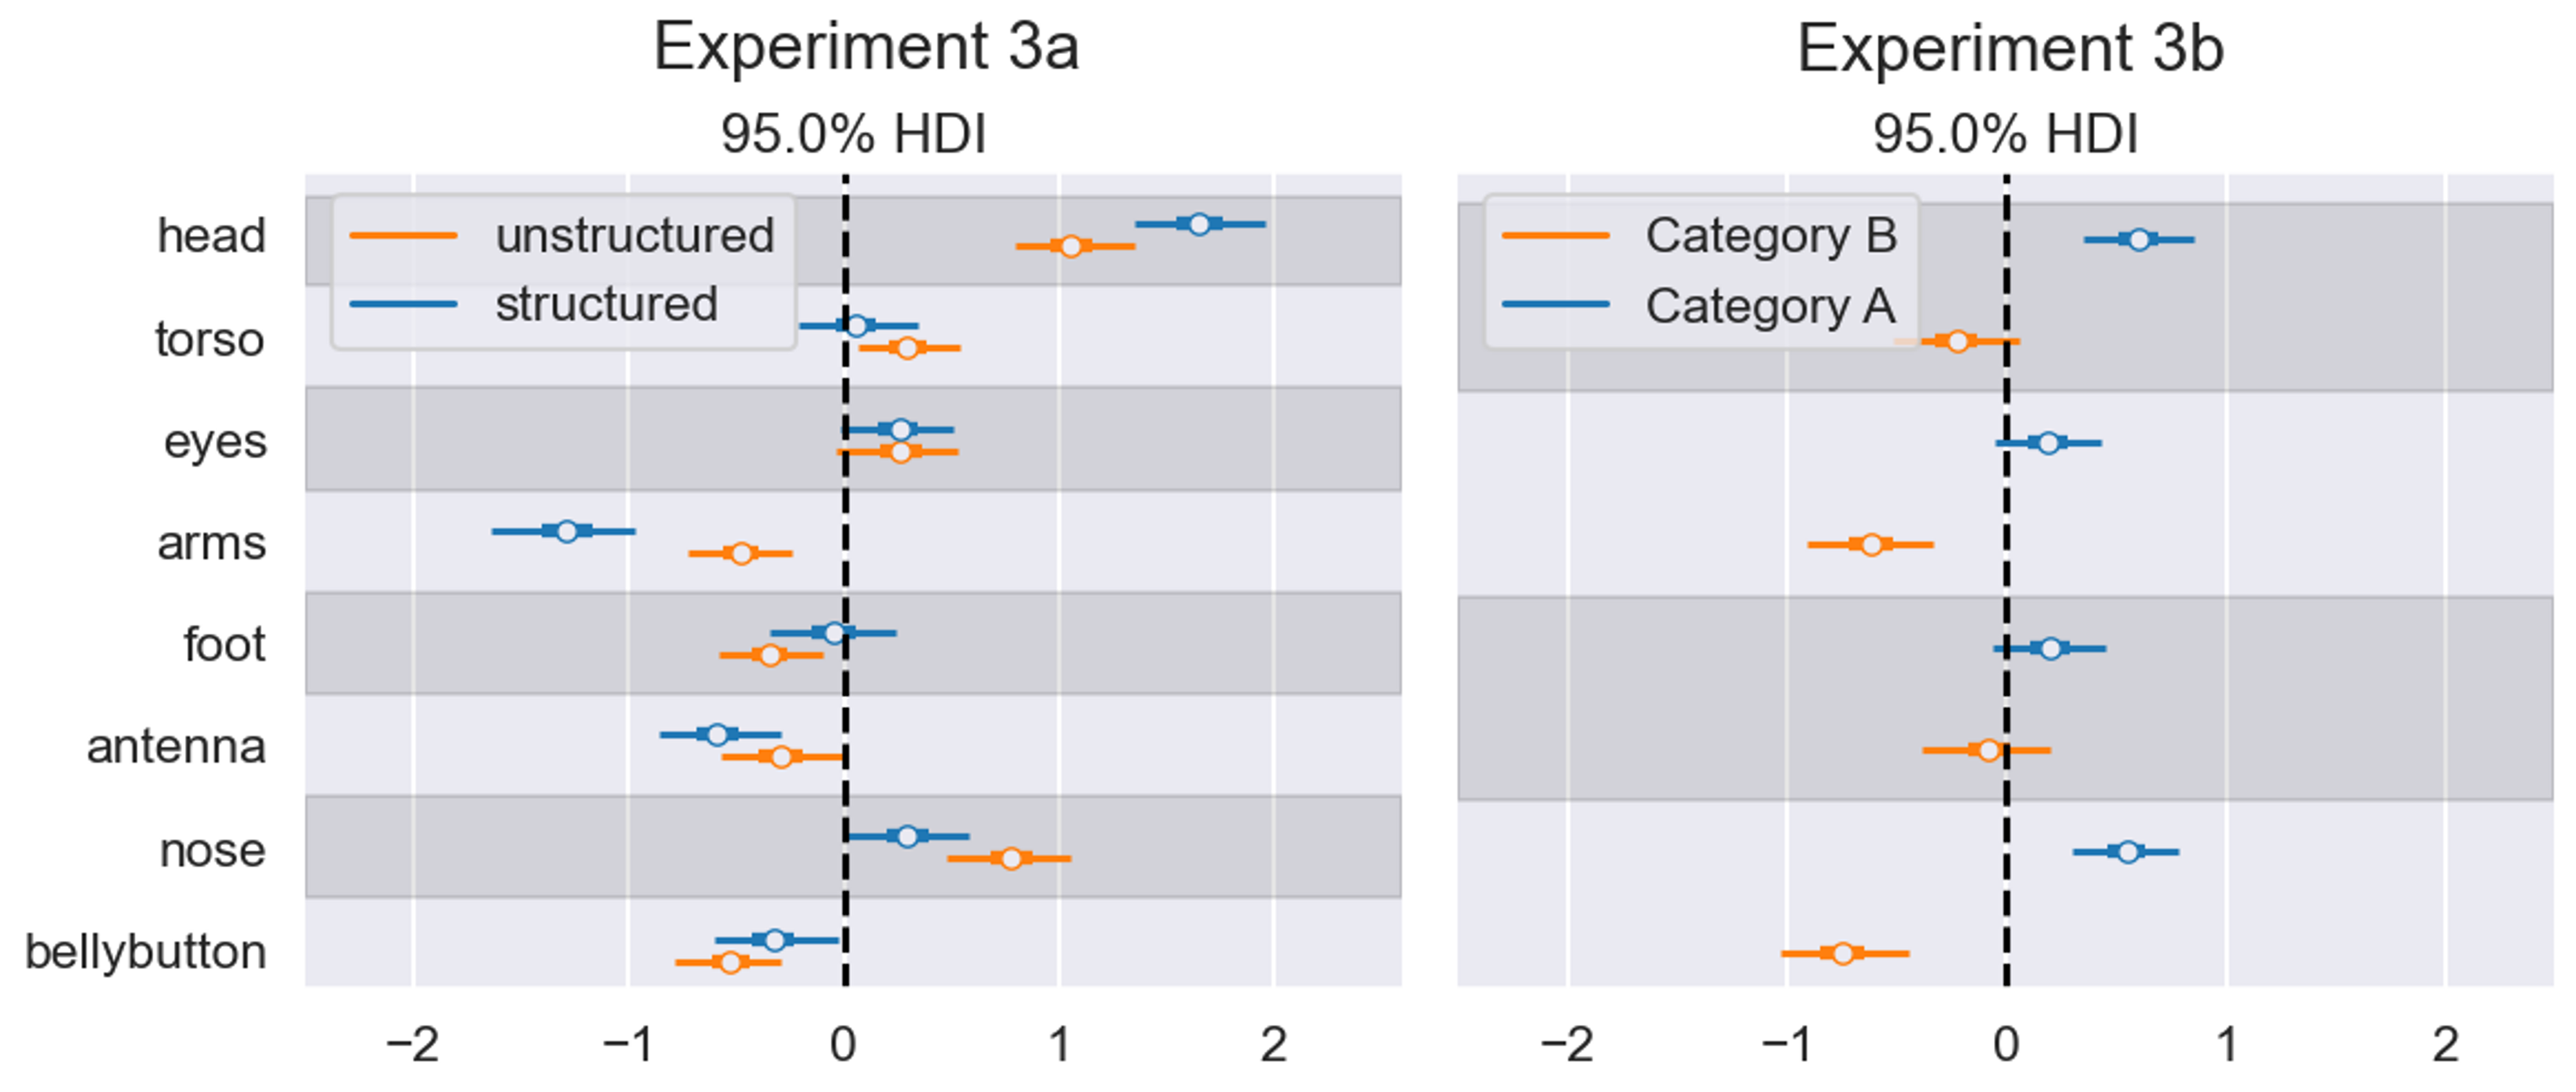
\includegraphics[width = \textwidth]{chapter_notebooks/chapter_4/figures/feat_importances.png}
    \caption{Relative weights placed by participants to categorize test stimuli. Values above 0 indicate features that are category diagnostic (i.e. remained consistent during exposure) are chosen more often to categorize whereas values below 0 indicate features that are category non-diagnostic (i.e. changed frequently) are used to categorize.}
    \label{fig:feat-importances}
\end{figure}

As seen in Figure \ref{fig:feat-importances}, some features are grouped together for being temporally consistent whereas some features are grouped together for being temporally inconsistent. Interestingly, this is true even in the unstructured case. Regardless of the temporal exposure, participants will group aliens together if they have the same head color or nose shape. On average, features that were chosen to be category diagnostic for Category A participants in experiment 3b (head, eyes, foot, and nose), were inherently grouped together for sharing feature values. Whereas features that were chosen to be category diagnostic for Category B participants in experiment 3b (torso, arms, antenna, bellybutton) were inherently grouped together if the did \textit{not} share feature values. While this analysis does not address covariances among features, it provides a possible explanation for patterns in Experiment 3b -- visual features carry different weights in categorization. Based on their weights, attention may be drawn to them either for being temporally consistent or for being temporally inconsistent. Future modeling will aim to assess whether baseline attention weights modulate the effect of order of presentation in implicit categorization tasks. 